documentclass{article}
\usepackage{amsmath}
\usepackage{tikz}
\usetikzlibrary{patterns}
\usepackage{pgfplots}

\begin{document}

\begin{figure}[h]
  \centering
    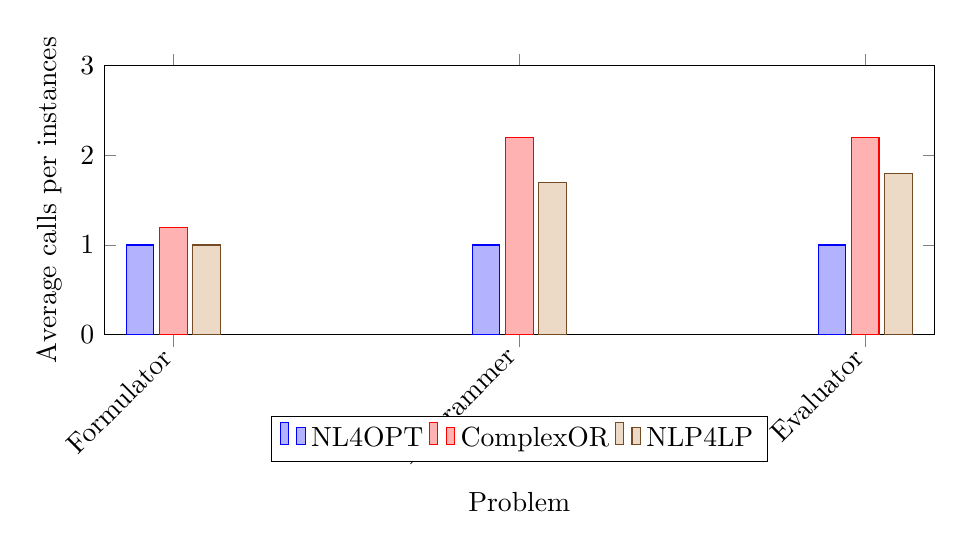
\begin{tikzpicture}
      \begin{axis}[
          ybar,
          width=\textwidth,
          height=5cm,
          legend style={
            at={(0.5,-0.3)},
            anchor=north,
            legend columns=-1,
          },
          ylabel={Average calls per instances},
          symbolic x coords={Formulator, Programmer, Evaluator},
          xtick=data,
          nodes near coords align={vertical},
          ymin=0,
          ymax=3,
          x tick label style={rotate=45,anchor=east},
          scaled x ticks=false,
          xlabel={Problem},
        ]
        \addplot coordinates {(Formulator,1) (Programmer,1) (Evaluator,1)};
        \addplot coordinates {(Formulator,1.2) (Programmer,2.2) (Evaluator,2.2)};
        \addplot coordinates {(Formulator,1) (Programmer,1.7) (Evaluator,1.8)};
        \legend{NL4OPT,ComplexOR,NLP4LP}
      \end{axis}
    \end{tikzpicture}
\end{figure}
\end{document}